\scanpage{123}
4) \mbox{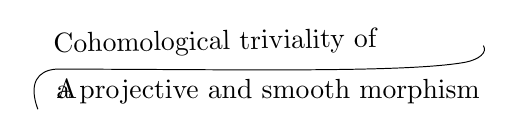
\begin{tikzpicture}[x=1em,y=1em,baseline=(b.base)]
\node[anchor=base west,inner sep=0] (b) at (0,0) {\uline{\rlap{\deleted{A}}\handwritten{a} projective and smooth morphism}};
\node[anchor=base west,inner sep=0,rotate=1] at (-.1,1.65) {\inserted{\handwritten{\uline{Cohomological triviality of}}}};
\draw[line width=.35pt] (-.65,-.4) .. controls (-1.0,.55) and (-.65,1.0) .. (.0,1.05) .. controls (6,1.05) and (12.6,.9) .. (14.8,1.3) .. controls (15.3,1.4) and (15.6,1.65) .. (15.45,1.9);
\end{tikzpicture}} $f:X\handwritten{\longrightarrow}Y$ \uline{of schemes} (corresponding intuitively to a fibration over $Y$ with nonsingular projective varieties as fibres). \deleted{is always cohomol\unsure{o}gically} \mbox{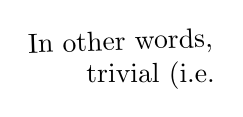
\begin{tikzpicture}[x=1em,y=1em,baseline=(b.base)]
\node[anchor=base west,inner sep=0] (b) at (0,0) {\deleted{trivial (i.e.}};
\node[anchor=base west,inner sep=0,rotate=2] at (-2.1,1.05) {\inserted{\handwritten{In other words,}}};
\end{tikzpicture}} \rlap{\deleted{t}}\handwritten{T}he Leray spectral sequence for $\handwritten{\unsure{\ell|l}}$-adic cohomology - or with real coeffi\deleted{\unsure{s}}cients in the case of the base field $C$\deleted{)} - \mbox{\resizebox{\linewidth}{!}{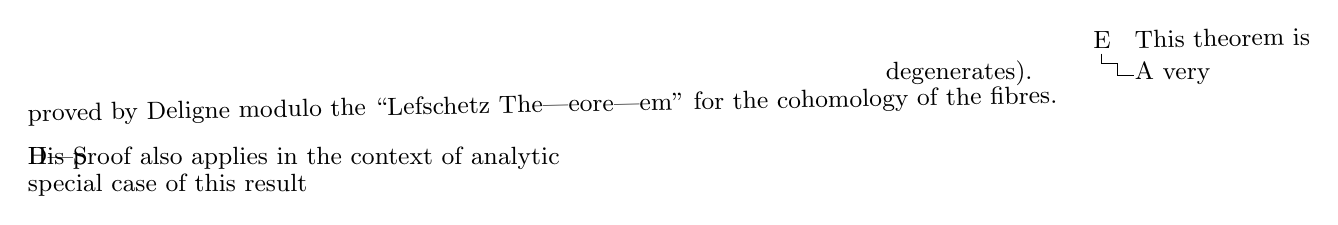
\begin{tikzpicture}[x=1em,y=1em,font=\small]
\node[anchor=base west,inner sep=0] at (31,0) {degenerates\deleted{)}.};
\node[anchor=base west,inner sep=0] at (40,0) {\deleted{A very}};
\node[anchor=base west,inner sep=0] at (38.5,1.15) {\handwritten{\deleted{\unsure{E}}}};
\draw[line width=.45pt] (38.8,.95) -- (38.8,.6) -- (39.4,.6) -- (39.4,.15) -- (40,.15);
\node[anchor=base west,inner sep=0,rotate=1] at (40,1.15) {\inserted{\handwritten{This theorem is}}};
\node[anchor=base west,inner sep=0,rotate=1] at (0,-1.5) {\inserted{\handwritten{proved by Deligne modulo the ``Lefschetz Th\unsure{e|e}or\unsure{e|e}m'' for the cohomology of the fibres.}}};
\node[anchor=base west,inner sep=0] at (0,-3.05) {\rlap{\deleted{\unsure{D|S}}}\handwritten{H}is proof also applies in the context of analytic};
\node[anchor=base west,inner sep=0] at (0,-4.05) {\deleted{special case of this result}};
\end{tikzpicture}}} varieties, for a complex analytic fibration with compact Kähler fibres. A very special case of this theorem, relating to the case where the local system of the cohomology of the fibres was trivial, constitute\mbox{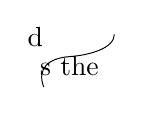
\begin{tikzpicture}[x=1em,y=1em,baseline=(b.base)]
\node[anchor=base west,inner sep=0] (b) at (0,0) {\deleted{s} the};
\node[anchor=base west,inner sep=0] at (-.45,1.05) {\inserted{d}};
\draw[line width=.35pt] (.15,-.4) .. controls (-.1,.25) and (.3,.65) .. (1.1,.7) .. controls (1.8,.75) and (2.7,1) .. (2.7,1.5);
\end{tikzpicture}} main result of Blanchard's thesis; but Blanchard's hypothesis is satisfied in almost no interesting case in geometry. Deligne's proof is of course different from that of Blanchard, which Deligne did not know.

Already from the transcendental point of view, the interest of Deligne's result \deleted{in topology} for the topology of analytic varieties is evident. In the writer's view however, it is its implications in abstract algebraic geometry,and in the long term, for number theory, that are the most interesting\handwritten{,} \deleted{For example, th\unsure{e|e}} \deleted{and} \rlap{\deleted{\unsure{i}}}\handwritten{I}t is moreover arithmet\unsure{\rlap{c}i|\rlap{i}c}\unsure{\rlap{i}c|\rlap{c}i}al considerations that had led the \mbox{
\begin{tikzpicture}[x=1em,y=1em,baseline=(b.base)]
\node[anchor=base west,inner sep=0] (b) at (0,0) {\deleted{writer}};
\node[anchor=base west,inner sep=0,rotate=1] at (-.05,1.1) {\inserted{\handwritten{referee}}};
\end{tikzpicture}} to communicate to Deligne \deleted{the conjecture} the preceding statement \unsure{\rlap{s}a|\rlap{a}s}s a conjecture. Thanks to Deligne's theorem, one can see for example that the R\rlap{\deleted{e}}\handwritten{i}\rlap{\deleted{i}}\handwritten{e}mann-Weil hypotheses in Diophantine geometry, interpreted in terms of the properties of a Frobenius endomorphism on $\handwritten{\unsure{\ell|l}}$-adic cohomology, \deleted{remain valid under a} imply analogous properties in the case of twist\unsure{\rlap{d}e|\rlap{e}d}d coefficients (which may have arbitrary singularities, moreover). Deligne's theorem will be one of the \mbox{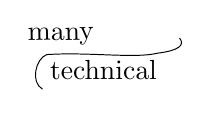
\begin{tikzpicture}[x=1em,y=1em,baseline=(b.base)]
\node[anchor=base west,inner sep=0] (b) at (0,0) {technical};
\node[anchor=base west,inner sep=0,rotate=1] at (-.8,1.4) {\inserted{\handwritten{many}}};
\draw[line width=.35pt] (-.25,-.35) .. controls (-.7,-.1) and (-.5,.75) .. (-.1,.9) .. controls (1.4,1.0) and (3.1,.75) .. (3.9,.95) .. controls (4.7,1.05) and (4.9,1.25) .. (4.7,1.5);
\end{tikzpicture}} ingredients \mbox{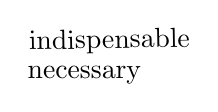
\begin{tikzpicture}[x=1em,y=1em,baseline=(b.base)]
\node[anchor=base west,inner sep=0] (b) at (0,0) {\deleted{necessary}};
\node[anchor=base west,inner sep=0,rotate=1] at (.05,1.05) {\inserted{\handwritten{indispensable}}};
\end{tikzpicture}} for developing the ``theory of motives'', which \handwritten{will} \rlap{\deleted{\unsure{i}}}\handwritten{\unsure{b}}\rlap{\deleted{\unsure{s}}}\handwritten{e}
% archive sheet number: 122
